%!TEX root = IntensionalSemantics.tex
\chapter{Conditionals}\label{cha:conditionals} % (fold)

\chapterprecishere{We integrate conditionals into the semantics of modal expressions that we are developing. We show that the material implication analysis and the strict implication analysis are inferior to the restrictor analysis. Our discussion will remain focussed on some simple questions and we refer you to the rich literature on conditionals for further topics.}

\minitoc

\section{The Material Implication Analysis}

Consider the following example:

\ex. If I am healthy, I will come to class.

The simplest analysis of such conditional constructions is the so-called \term{material implication} analysis,\footnote{Quoth the Stoic philosopher Philo of Megara: ``a true conditional is one which does not have a true antecedent and a false consequent'' (according to \citet[II, 110--112]{sextus-empiricus:200:outlines}).} which treats \expression{if} as contributing a truth-function operating on the truth-values of the two component sentences (which are called the \term{antecedent} and \term{consequent} \dash from Latin \dash or \term{protasis} and \term{apodosis} \dash from Greek). The lexical entry for \expression{if} would look as follows:

\ex.\label{ex:material} \marginnote{Note that as a truth-functional connective, this \expression{if} does not vary its denotation depending on the evaluation world. It's its arguments that vary with the evaluation world.}$\sv{\mbox{if}} = \lambda u \in D_t.\ \lambda v \in D_t.\ u=0 \mbox{ or } v=1.$

Applied to example in \LLast, this semantics would predict that the example is false just in case the antecedent is true, I am healthy, but the consequent false, I do not come to class. Otherwise, the sentence is true. We will see that there is much to complain about here. But one should realize that under the assumption that \expression{if} denotes a truth-function, \emph{this one} is the most plausible candidate.

\citet{suber:1997:material} does a good job of persuading (or at least trying to persuade) recalcitrant logic students:

\begin{quote}
	
	After saying all this, it is important to note that material implication does conform to some of our ordinary intuitions about implication. For example, take the conditional statement, \expression{If I am healthy, I will come to class.} We can symbolize it: H $\supset$ C.\footnote{The symbol $\supset$ which Suber uses here is called the ``horseshoe''. We have been using the right arrow $\rightarrow$ as the symbol for implication. We think that this is much preferable to the confusing horseshoe symbol. There is an intimate connection between universal quantification, material implication, and the subset relation, usually symbolized as $\subset$, which is the other way round from the horseshoe. The horseshoe can be traced back to the notation introduced by \citet{peano:1889:nova}, a capital C standing for `conseguenza' facing backwards. The C facing in the other (more ``logical'') direction was actually introduced first by \citet{gergonne:1817:essai}, but didn't catch on.}
	
	The question is: when is this statement false? When will I have broken my promise? There are only four possibilities:
	
	\begin{center}
		\begin{tabular}
			{c|c||c} H & C & H$\supset$ C\\
			\hline T & T & ?\\
			T & F & ?\\
			F & T & ?\\
			F & F & ? 
		\end{tabular}
	\end{center}

\begin{itemize}
		
		\item In case \#1, I am healthy and I come to class. I have clearly kept my promise; the conditional is true. 
		\item In case \#2, I am healthy, but I have decided to stay home and read magazines. I have broken my promise; the conditional is false. 
		\item In case \#3, I am not healthy, but I have come to class anyway. I am sneezing all over you, and you're not happy about it, but I did not violate my promise; the conditional is true. 
		\item In case \#4, I am not healthy, and I did not come to class. I did not violate my promise; the conditional is true. 

\end{itemize}
%	
But this is exactly the outcome required by the material implication. The compound is only false when the antecedent is true and the consequence is false (case \#2); it is true every other time.

\end{quote}
%
Despite the initial plausibility of the analysis, it cannot be maintained. Consider this example:

\ex. \label{earthquake}If there is a major earthquake in Cambridge tomorrow, my house will collapse.

If we adopt the material implication analysis, we predict that \Last will be false just in case there is indeed a major earthquake in Cambridge tomorrow but my house fails to collapse. This makes a direct prediction about when the negation of \Last should be true. A false prediction, if ever there was one:

\ex. \a. \label{neg-earthquake}It's not true that if there is a major earthquake in Cambridge tomorrow, my house will collapse. 
\b. $\not\equiv$ There will be a major earthquake in Cambridge tomorrow, and my house will fail to collapse.

Clearly, one might think that \Last[a] is true without at all being committed to what the material implication analysis predicts to be the equivalent statement in \Last[b]. This is one of the inadequacies of the material implication analysis.

These inadequacies are sometimes referred to as the ``paradoxes of material implication''. But that is misleading. As far as logic is concerned, there is nothing wrong with the truth-function of material implication. It is well-behaved and quite useful in logical systems. What is arguable is that it is not to be used as a reconstruction of what conditionals mean in natural language.

\begin{exercise}
  Under the assumption that \emph{if} has the meaning in \ref{ex:material}, calculate the truth-conditions predicted for \Next:

\ex. \a. No student will succeed if he goofs off.
\b. No student $\lambda x$ (if $x$ goofs off, $x$ will succeed)

State the predicted truth-conditions in words and evaluate whether they correspond to the actual meaning of \Last.
\eex
\end{exercise}

A 
%
\marginpar{
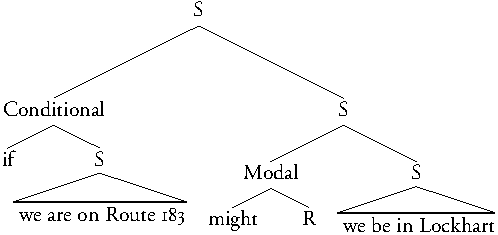
\includegraphics[width=\marginparwidth]{lockhartmight-a}\figcaption{LF A for \ref{lockhartmight}}}
%
\marginpar{
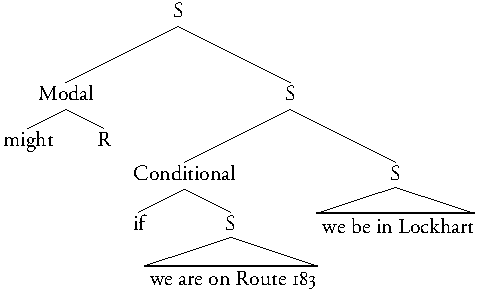
\includegraphics[width=\marginparwidth]{lockhartmight-b}\figcaption{LF B for \ref{lockhartmight}}}
% 
problem that is not often raised for the material implication analysis is how badly it interacts with the analysis of modal expressions, once we look at sentences involving both a conditional clause and a modal. Consider:

\ex. \label{lockhartmight}If we are on Route 183, we might be in Lockhart now.

\ex. \label{fern}If you keep this fern dry, it cannot grow.

We need to consider two possible LFs for these sentences, depending on whether wider scope is given to the modal or to the conditional clause. For example, in the margin you see LFs A and B for \ref{lockhartmight}.

\begin{wrapfigure}{l}{40mm}
  \begin{center}
    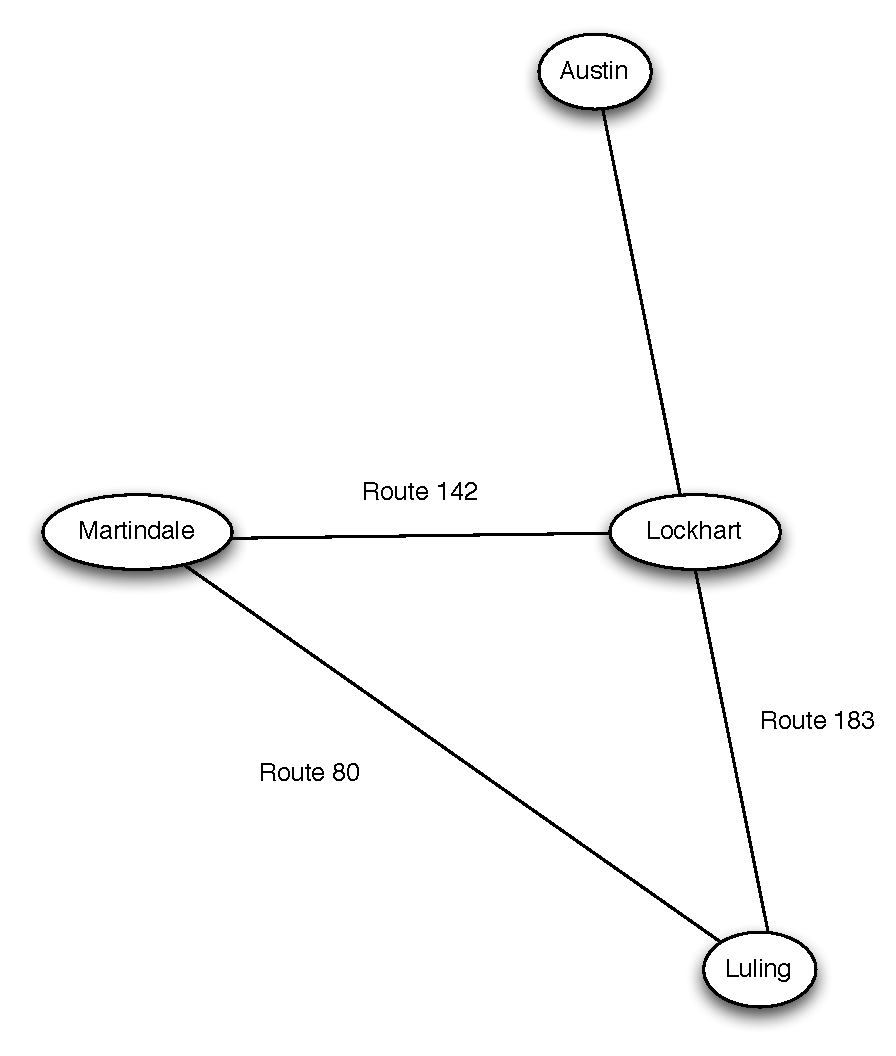
\includegraphics[width=40mm]{183}
  \end{center}
  \caption{A schematic map of the relevant area in Texas}
\end{wrapfigure}
%
The reading for \ref{lockhartmight} we have in mind is an epistemic one; imagine for instance that \ref{lockhartmight} is uttered in a car by Mary to Susan, while Susan is driving and Mary is looking at a map. The information provided by the map, together with other background knowledge, constitutes the relevant context for the modal \expression{might} here. The accessibility relation is roughly this:

\ex. $\lambda w.\ \lambda w'.\ w'$ is compatible with what the map says in $w$ and what Mary knows about the geography of the relevant area in $w$.

Let's suppose \ref{lockhartmight} is uttered in the actual world $w_0$ and we are interested in its truth-value at this world. We now proceed to show that neither of the LFs A and B represent the intuitively natural meaning of \ref{lockhartmight} if we assume the material implication analysis of \expression{if}.

Consider first LF A. There are two respects in which the predicted truth-conditions for this LF deviate from intuitive judgment. First, suppose that Susan and Mary are not on Route 183 in $w_0$. Then \ref{lockhartmight} is predicted to be true in $w_0$, regardless of the geographical facts, e.g. even if Lockhart is nowhere near Route 183. This is counterintuitive. Imagine the following quite sensible dialogue:

\ex. Mary: If we are on Route 183, we might be in Lockhart now.\\
Susan (stops the car and looks at the map): You are wrong. Look here, Route 183 doesn't run anywhere near Lockhart.

If Mary concedes Susan's claim that Route 183 doesn't go through Lockhart, she has to also concede that her original assertion was false. It wouldn't do for her to respond: ``I know that 183 runs about 10 miles east of Lockhart, but maybe we are not on Route 183, so I may still be right.'' Yet we predict that this should be a reasonable way for her to defend \ref{lockhartmight}.

A second inadequacy is this: we predict that the truth of the consequent of \ref{lockhartmight} is a sufficient condition for the truth of \ref{lockhartmight} as a whole. If this were right, it would take very little for \ref{lockhartmight} to be true. As long as the map and the rest of Mary's knowledge in $w_0$ don't rule out the possibility that they are in Lockhart, \expression{we might be in Lockhart} will be true in $w_0$ \dash regardless, once again, of whether Lockhart is anywhere near 183. It should therefore be reasonable for Mary to continue the dialogue in \Last with the rejoinder: ``But how can you be so sure we are not in Lockhart?'' According to intuitive judgment, however, this would not be a pertinent remark and certainly would not help Mary defend \ref{lockhartmight} against Susan's objection.

Now let's look at LF B, where the modal has widest scope. Given the material implication analysis of \expression{if}, this is predicted to mean, in effect: ``It might be the case that we are either in Lockhart or not on Route 183''. This truth-condition is also far too easy to satisfy: All it takes is that the map and the rest of Mary's knowledge in $w_0$ are compatible with Mary and Susan not being on Route 183, or that they are compatible with their being in Lockhart. So as long as it isn't certain that they are on Route 183, Mary should be justified in asserting \ref{lockhartmight}, regardless, once again, of her information about the relative location of Lockhart and Route 183.

\begin{exercise}
	Show that similar difficulties arise for the analysis of \ref{fern}. \eex 
\end{exercise}

\section{The Strict Implication Analysis}

Some of the problems we encountered would go away if we treated \expression{if} as introducing a modal meaning. The simplest way to do that would be to treat it as a universal quantifier over possible worlds. \expression{If p, q} would simply mean that the set of $p$-worlds is a subset of the $q$-worlds. This kind of analysis is usually called \term{strict implication}. The difference between \expression{if} and \expression{must} would be that \expression{if} takes an overt restrictive argument. Here is what the lexical entry for \expression{if} might look like:

\ex. $\sv{\mbox{if}}^{w,g} = \lambda p \in D_{\angles{s,t}}.\ \lambda q \in D_{\angles{s,t}}.\ \forall w'\co p(w')=1 \rightarrow q(w')=1.\\[6pt]
(\mbox{in set talk: } p \subseteq q)$

Applied to \ref{earthquake}, we would derive the truth-conditions that \ref{earthquake} is true iff all of the worlds where there is a major earthquake in Cambridge tomorrow are worlds where my house collapses.

We immediately note that this analysis has the same problem of non-contingency that we faced with one of our early attempts at a quantificational semantics for modals like \expression{must} and \expression{may}. The obvious way to fix this here is to assume that \expression{if} takes a covert accessibility function as one of its arguments. The antecedent clause then serves as an additional restrictive device. Here is the proposal:

\ex. $\sv{\mbox{if}}^{w,g} = \lambda R \in D_{\angles{s,\angles{s,t}}}.\ \lambda p\in D_{\angles{s,t}}.\ \lambda q\in D_{\angles{s,t}}.\\
\null\hfill \forall w'\co \left( R(w)(w')=1\ \&\ p(w')=1 \right) \rightarrow q(w')=1.\\[6pt]
(\mbox{in set talk: }R(w)\cap p \subseteq q)$

If we understand \ref{earthquake} as involving an epistemic accessibility relation, it would claim that among the worlds epistemically accessible from the actual world (i.e. the worlds compatible with what we know), those where there is a major earthquake in Cambridge tomorrow are worlds where my house collapses. This would appear to be quite adequate \dash although potentially traumatic to me.

\begin{exercise}
	
	Can you come up with examples where a conditional is interpreted relative to a non-epistemic accessibility relation? \eex
\end{exercise}

\begin{exercise}
	
	What prediction does the strict implication analysis make about the negated conditional in \ref{neg-earthquake}? \eex
\end{exercise}

%
%\absatz [what about deontic accessibility? what about compatibility
%presupposition?]
%
What happens when we let this analysis loose on \ref{lockhartmight}? We again need to assess two LFs depending on the relative scope of \expression{if} and \expression{might}. Both LFs would have two covert variables over accessibility relations, one for \expression{if} and one for \expression{might}. Before we can assess the adequacy of the two candidate analyses, we need to decide what the contextually salient values for the accessibility relations might be. One would think that the epistemic accessibility relation that we have already encountered is the most likely value, and in fact for both variables.

Next, 
%
\marginpar{
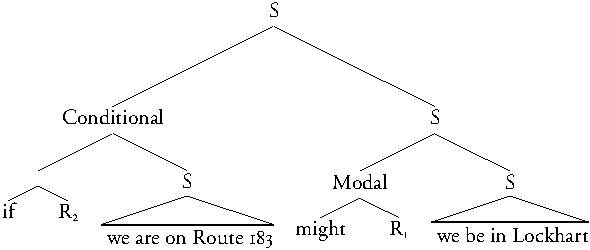
\includegraphics[width=\marginparwidth]{lockhartmight-aprime}\figcaption{LF A$'$ for \ref{lockhartmight}}}
%
\marginpar{
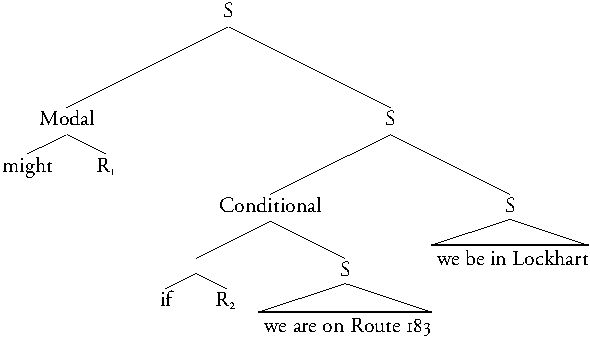
\includegraphics[width=\marginparwidth]{lockhartmight-bprime}\figcaption{LF B$'$ for \ref{lockhartmight}}}
% 
we need to consider the particular epistemic state that Mary is in. By assumption, Mary does not know where they are. Nothing in her visual environment helps her figure out where they are. She does see from the map that if they are on Route 183, one of the towns they might be in is Lockhart. But she doesn't know whether they are on Route 183. Even if they \emph{are} on 183, she doesn't know that they are and her epistemic state would still be what it is: one of being lost.

Consider then LF A$'$, with the modal in the scope of the conditional. Here, we derive the claim that all worlds $w'$ compatible with what Mary knows in $w$ and where they are on 183 are such that some world $w''$ compatible with what Mary knows in $w'$ is such that they are in Lockhart. Is that adequate? Not really. We have just convinced ourselves that whether they are on 183 or not has no relevant influence on Mary's epistemic state, since she wouldn't know it either way. But that means that our analysis would predict that \ref{lockhartmight} is true as long as it is possible as far as Mary knows that they are in Lockhart. Whether they are on 183 or not doesn't change that. So, we would expect \ref{lockhartmight} to not be distinct in truth-value from something like:

\ex. If we are on the Route 80, we might be in Lockhart.

But that is not right \dash Mary knows quite well that if they are on the Route 80, they cannot be in Lockhart. 

Turning to LF B$'$, with the modal having widest scope, doesn't help us either. Here, we would derive the claim that it is compatible with what Mary knows that from being on 183 it follows (according to what she knows) that they are in Lockhart. Clearly, that is not what \ref{lockhartmight} means. Mary doesn't consider it possible that if they are on 183, she knows that they are in Lockhart. After all, she's well aware that she doesn't know where they are.

\section{\expression{If}-Clauses as Restrictors}

The problem we have encountered here with the interaction of an \expression{if}-clause and the modal operator \expression{might} is similar to others that have been noted in the literature. Most influentially, David Lewis in his paper ``Adverbs of Quantification'' showed how hard it is to find an adequate analysis of the interaction of \expression{if}-clauses and \term{adverbs of quantification} like \expression{never, rarely, sometimes, often, usually, always}. Lewis proposed that in the cases he was considering, the adverb is the only operator at work and that the \expression{if}-clause serves to restrict the adverb. Thus, it has much the same function that a common noun phrase has in a determiner-quantification. %\marginpar{\centering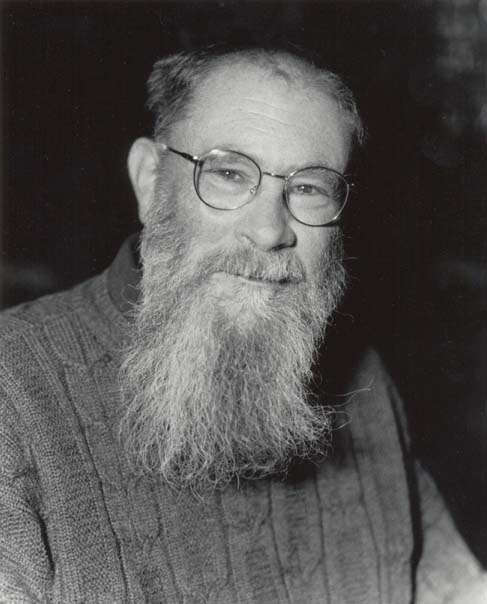
\includegraphics[height=1in]{lewis.jpg}\\ {\tiny \href{http://en.wikipedia.org/wiki/David_Lewis_(philosopher)}{David Lewis}}}

\begin{quote}
	
	The \expression{if} of our restrictive \expression{if}-clauses should not be regarded as a sentential connective. It has no meaning apart from the adverb it restricts. The \expression{if} in \expression{always if \ldots, \ldots, sometimes if \ldots, \ldots}, and the rest is on a par with the non-connective \expression{and} in \expression{between \ldots and \ldots}, with the non-connective \expression{or} in \expression{whether \ldots or \ldots}, or with the non-connective \expression{if} in \expression{the probability that \ldots if \ldots}. It serves merely to mark an argument-place in a polyadic construction. \cite[11]{lewis:1975:adverbs}

\end{quote}
%
Building on Lewis' insight, Kratzer argued for a uniform treatment of \expression{if}-clauses as restrictors. She claimed that 

\begin{quote}
	
	the history of the conditional is the story of a syntactic mistake. There is no two-place \expression{if \ldots then} connective in the logical forms of natural languages. \expression{If}-clauses are devices for restricting the domains of various operators. \citep{kratzer:1986:conditionals}
\end{quote}
%
Let us repeat this:

\ex. \extitle{Kratzer's Thesis}\\[3pt]
\expression{If}-clauses are devices for restricting the domains of various operators.

Kratzer's Thesis gives a unified picture of the semantics of conditional clauses. Note that it is not meant to supplant previous accounts of the meaning of conditionals. It just says that what those accounts are analyzing is not the meaning of \expression{if} itself but the meaning of the operators that \expression{if}-clauses restrict. 

Let us see how this idea helps us with our Lockhart-sentence. The idea is to deny that there are two quantifiers over worlds in \ref{lockhartmight}. Instead, the \expression{if}-clause merely contributes a further restriction to the modal \expression{might}. In effect, the modal is not quantifying over \emph{all} the worlds compatible with Mary's knowledge but only over those where they are on Route 183. It then claims that at least some of those worlds are worlds where they are in Lockhart. We cannot anymore derive the problematic conclusion that it should also be true that if they are on the Route 80, they might be in Lockhart. In all, we have a good analysis of what \ref{lockhartmight} means.

What 
%
\marginpar{
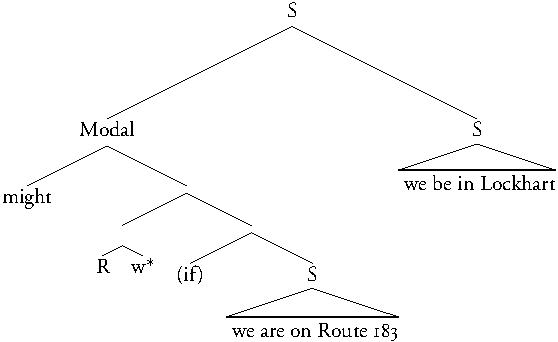
\includegraphics[width=\marginparwidth]{lockhartlf-final}\figcaption{LF C for \ref{lockhartmight}}}
%
we don't yet have is a compositional calculation. What does it mean in structural terms for the \expression{if}-clause to be restricting the domain of the modal? We will assume a structure as in LF C. Here, the \expression{if}-clause is the sister to what used to be the covert set-of-worlds argument of the modal. As you can see, we have chosen the variant of the semantics for modals that was discussed in Section \ref{techvariant}. The idea now is that the two restrictive devices work together: we just feed to the modal the \emph{intersection} of (i) the set of worlds that are $R$-accessible from the actual world, and (ii) the set of worlds where they are on Route 183.

\begin{exercise}
	
	To make the composition work, we need to be able to intersect the set of accessible worlds with the antecedent proposition. This could be done in two ways: (i) a new composition principle, which would be a slight modification of the \term{Predicate Modification} rule, (ii) give \expression{if} a functional meaning that accomplishes the intersection. Formulate such a meaning for \expression{if}.
	
	Alternatively, we could do without the $w*$ device and instead give \expression{if} a meaning that takes a proposition $p$ and then modifies an accessibility relation to give a new accessibility relation, which is restricted to $p$-worlds. Formulate such a meaning for \expression{if}. \eex
\end{exercise}

What about cases like \ref{earthquake}, now? Here there is no modal operator for the \expression{if}-clause to restrict. Should we revert to treating \expression{if} as an operator on its own? Kratzer proposes that we should not and that such cases simply involve covert modal operators. % We will have nothing to say about that here.

%\bigskip\noindent [MUCH MORE TO COME \dots]

\newpage\section*{Supplementary Readings} \label{sec:suppl-read-conditionals}

\phantomsection \addcontentsline{toc}{section}{Supplemental Readings}

{\setlength{\parindent}{0pt}\setlength{\parskip}{6pt}

A short handbook article on conditionals:
\begin{bibentrylist}
	\item\bibentry{fintel:2009:hsk-conditionals}.
\end{bibentrylist}

Overviews of the philosophical work on conditionals:
\begin{bibentrylist}
	\item \bibentry{edgington:1995:conditionals}.
	\item \bibentry{bennett:2003:guide}.
\end{bibentrylist}

A handbook article on the logic of conditionals:
\begin{bibentrylist}
	\item \bibentry{nute:1984:conditional}.
\end{bibentrylist}

Three indispensable classics:
\begin{bibentrylist}
	\item \bibentry{lewis:1973:counterfactuals}.
	\item \bibentry{stalnaker:1968:theory}.
	\item \bibentry{stalnaker:1975:indicative}. 
\end{bibentrylist}

The Restrictor Analysis:
\begin{bibentrylist}
	\item \bibentry{lewis:1975:adverbs}. 
	\item \bibentry{kratzer:1986:conditionals}.
\end{bibentrylist}

The application of the restrictor analysis to the interaction of nominal quantifiers and conditionals:
\begin{bibentrylist}
	\item \bibentry{fintel:1998:qandif}.
	\item \bibentry{fintel-iatridou:2002:ifwhen}.
	\item \bibentry{higginbotham:2003:conditionals}.
	\item \bibentry{leslie:2009:unless}.
	\item \bibentry{huitink:2009:quantified-conditionals}.
\end{bibentrylist}

Syntax of conditionals:
\begin{bibentrylist}
  \item \bibentry{fintel:1994:thesis}, Chapter 3: ``Conditional Restrictors''
  \item \bibentry{iatridou:1993:then}.
	\item \bibentry{bhatt-pancheva:2006:conditionals}.
\end{bibentrylist}

A shifty alternative to the restrictor analysis:

\begin{bibentrylist}
  \item \bibentry{gillies:2009:truth-conditions}.
  \item \bibentry{gillies:2010:iffiness}.
\end{bibentrylist}

The Belnap alternative:

\begin{bibentrylist}
   \item \bibentry{belnap:1970:restricted}.
   \item \bibentry{belnap:1973:restricted}.
   \item \bibentry{fintel:2007:gurt-slides}.
   \item \bibentry{huitink:2008:thesis}, Chapters 1 and 2 give a nice summary of what we're covering in this class, while Chapter 5 is about the Belnap-method.
   \item \bibentry{huitink:2009:domain-conditionals}.
\end{bibentrylist}
  
%More references are given at the end of the next chapter.

}

% chapter conditionals (end)

